\documentclass[aspectratio=169,11pt]{beamer}

\usepackage[utf8]{inputenc}
\usepackage[T1]{fontenc}
\usepackage[spanish,es-nodecimaldot]{babel}
\usepackage{lmodern}
\usepackage{booktabs}
\usepackage{array}
\usepackage{ragged2e}
\usepackage{xcolor}

\definecolor{Navy}{HTML}{17243A}
\definecolor{Teal}{HTML}{087E83}
\definecolor{Coral}{HTML}{E56B52}
\definecolor{Gold}{HTML}{E6A23C}
\definecolor{Pale}{HTML}{F2F5F8}
\definecolor{Muted}{HTML}{607080}
\definecolor{Green}{HTML}{32866E}


\setbeamertemplate{frametitle}{%
  \vspace{.35em}\insertframetitle\par\vspace{.15em}%
  {\color{Teal}\rule{.12\paperwidth}{2pt}}\vspace{.2em}
}
\setlength{\leftmargini}{1.4em}
\setlength{\leftmarginii}{1.2em}

\newcommand{\tagline}[1]{{\color{Teal}\bfseries\small #1}}
\newcommand{\smallnote}[1]{{\color{Muted}\scriptsize #1}}
\newcommand{\strong}[1]{{\color{Navy}\bfseries #1}}
\newcommand{\evidence}[1]{\par\vspace{.25em}{\color{Muted}\scriptsize Evidencia revisada: #1}}

\title{Five Nights of Terror: ¿para quién es el juego?}
\subtitle{Especificidad (Bowman) y accesibilidad (HCI)}
\author{Proyecto de Interacción Humano--Computador}
\institute{Análisis del prototipo Unity + Flutter}
\date{}

\begin{document}

% 1
\begin{frame}[plain]
  \setbeamercolor{titlelike}{fg=white,bg=Navy}
  \begin{beamercolorbox}[wd=\paperwidth,ht=\paperheight,sep=1.2cm,center]{titlelike}
    {\LARGE\bfseries Five Nights of Terror: ¿para quién es el juego?}\par\vspace{.55cm}
    {\large Especificidad y accesibilidad en una interacción repartida entre PC, tablet y cámara}\par\vspace{.8cm}
    {\large Marcelo Torres y Anthony Briceño}\par\vspace{1cm}
  \end{beamercolorbox}
\end{frame}

% 2
\begin{frame}{El reto central del proyecto}
  \begin{columns}[T,onlytextwidth]
    \column{.55\textwidth}
      \tagline{Una experiencia repartida entre dos dispositivos}
      \vspace{.35em}
      \begin{itemize}
        \item En el \strong{PC}, el jugador vigila la escena 3D y a los animatrónicos.
        \item En la \strong{tablet}, elige tareas, resuelve minijuegos y atiende la caja musical.
        \item La cámara estima si la persona está mirando al PC.
      \end{itemize}
      \vspace{.15em}
      \begin{block}{Pregunta de evaluación}
        ¿Puede el jugador percibir, comprender y ejecutar las acciones necesarias sin que la cámara, el tiempo o el cambio de pantalla le impongan una barrera?
      \end{block}
    \column{.4\textwidth}
      \centering
      \vspace{.35cm}
      \fcolorbox{Teal}{Pale}{\parbox{.86\linewidth}{\centering\textbf{PC / Unity}\\ escena 3D + vigilancia\\[.4em]\Large $\updownarrow$\\[.4em]\textbf{Tablet / Flutter}\\ menú + minijuegos}}
      \vspace{.4cm}
      \smallnote{La atención cambia de un dispositivo al otro mientras la partida continúa.}
  \end{columns}
\end{frame}

% 3 NUEVA
\begin{frame}{Cómo se juega: tres amenazas, tres formas de defenderse}
  \small
  \begin{tabular}{>{\RaggedRight\arraybackslash}p{.14\linewidth} >{\RaggedRight\arraybackslash}p{.40\linewidth} >{\RaggedRight\arraybackslash}p{.34\linewidth}}
    \toprule
    \textbf{Amenaza} & \textbf{Qué la hace avanzar o atacar} & \textbf{Defensa del jugador}\\
    \midrule
    Freddy & Que el jugador \strong{no mire el PC}. Al llegar a su penúltimo punto, aguantar sin mirarlo el intervalo completo lo hace atacar. & Mirar la pantalla (cámara).\\[.35em]
    Vixy & Tareas de la tablet sin resolver: avanza con 3 pendientes y ataca con 4. & Resolver minijuegos a tiempo.\\[.35em]
    Puppet & Caja musical sin dar cuerda: al llegar a 0\,\% puede salir. & Mantener presionado en la tablet.\\
    \bottomrule
  \end{tabular}
  \vspace{.6em}

  \tagline{Tareas en la tablet:} cables, perillas, secuencias y ritmo.
  \smallnote{Regla de diseño: cada amenaza exige un tipo de atención distinto, y el jugador debe repartirla entre dos pantallas.}
\end{frame}

% 4
\begin{frame}{Capturas del prototipo en la tablet}
  \begin{columns}[T,onlytextwidth]
    \begin{column}{0.48\textwidth}
      \centering
      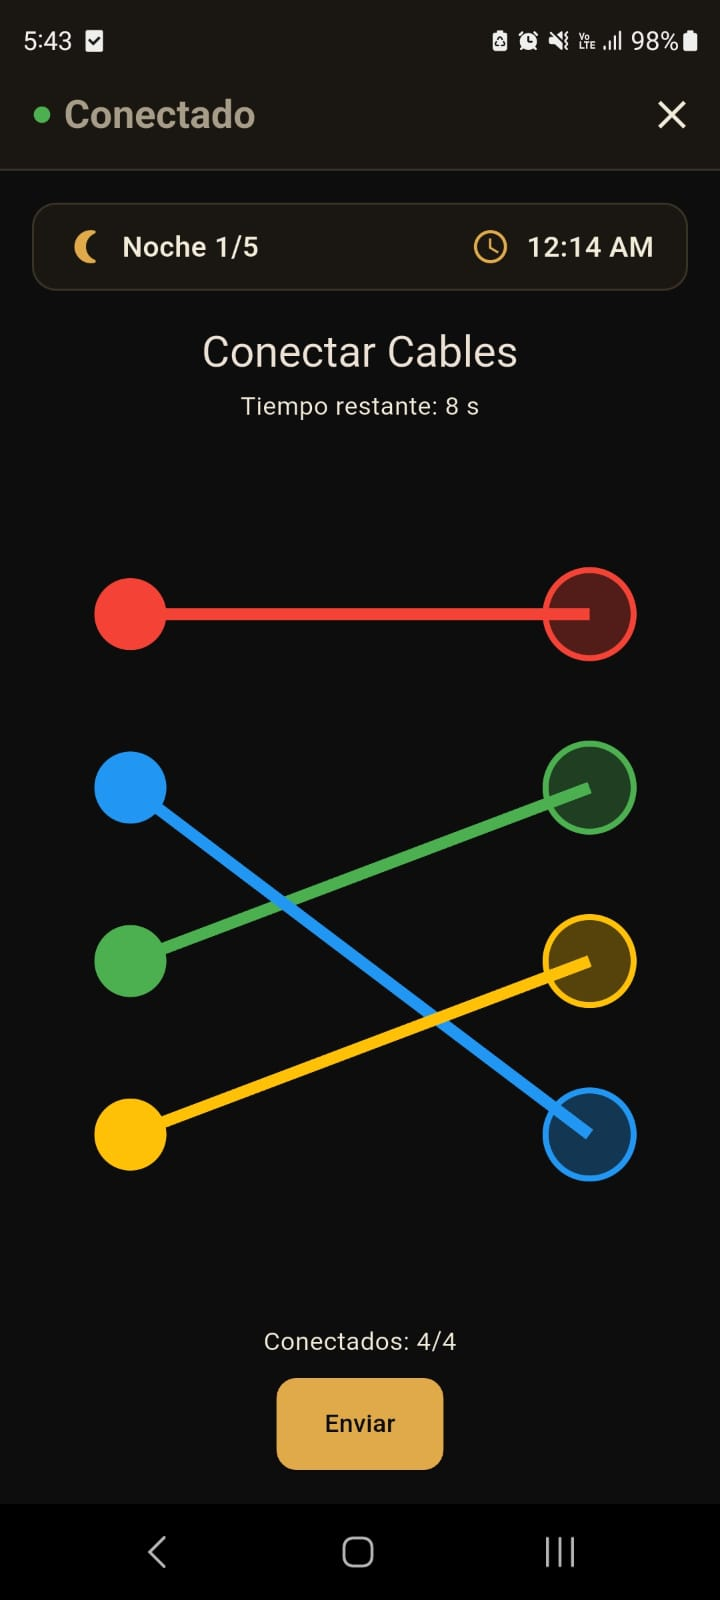
\includegraphics[width=\linewidth,height=0.62\textheight,keepaspectratio]{imagen-1.jpeg}

      \small Minijuego de conectar cables
    \end{column}
    \begin{column}{0.48\textwidth}
      \centering
      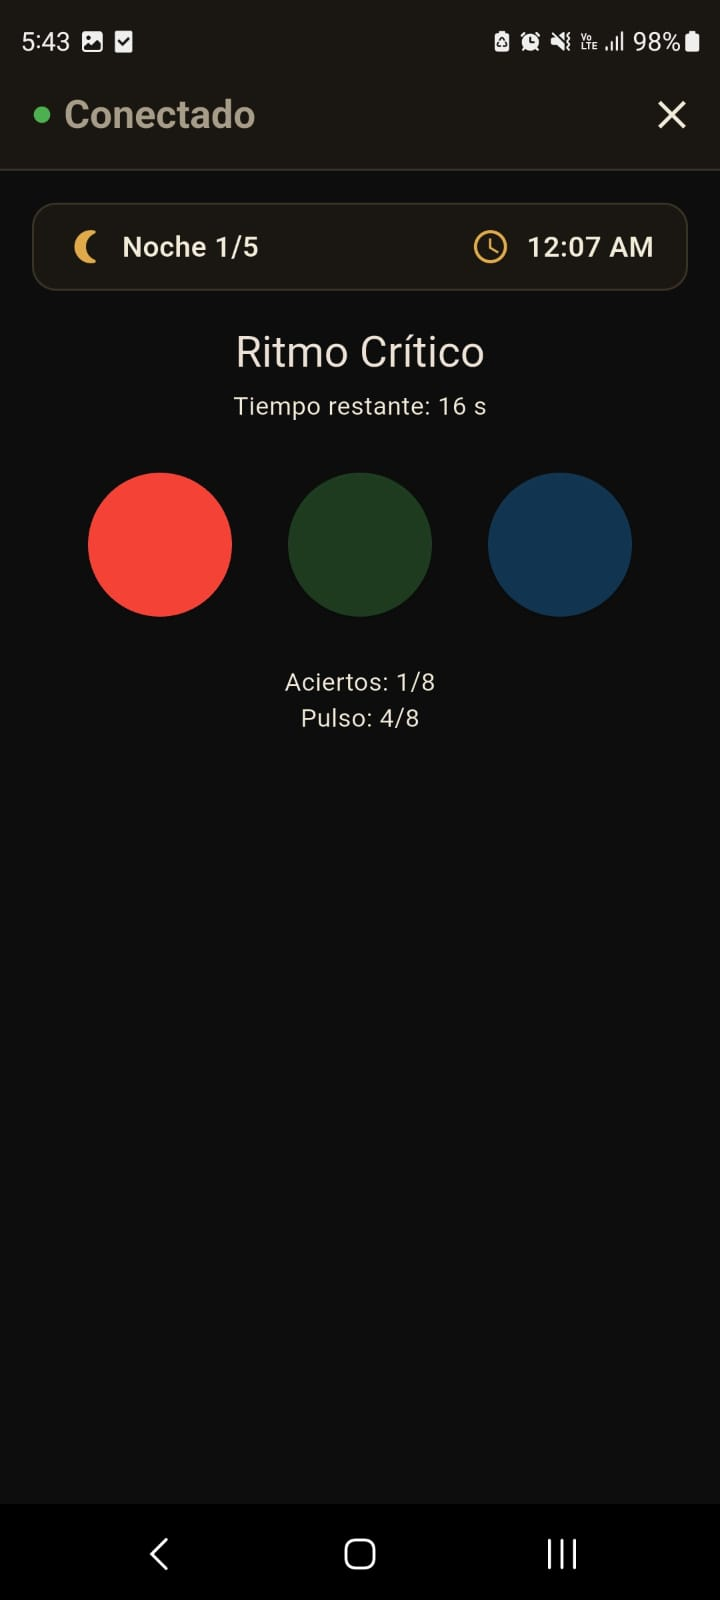
\includegraphics[width=\linewidth,height=0.62\textheight,keepaspectratio]{imagen-2.jpeg}

      \small Minijuego rítmico
    \end{column}
  \end{columns}
\end{frame}

% 5 NUEVA (reemplaza "Dos marcos")
\begin{frame}{Marco 1 (Bowman et al., 2006): la especificidad}
  \small
  \tagline{Idea del paper:} las técnicas genéricas fallan porque no se diseñaron para una situación concreta. Hay que acotar.
  \vspace{.4em}

  \begin{tabular}{>{\RaggedRight\arraybackslash}p{.17\linewidth} >{\RaggedRight\arraybackslash}p{.74\linewidth}}
    \toprule
    \textbf{Especificidad} & \textbf{En nuestro juego}\\
    \midrule
    Aplicación / dominio & Juego de terror y defensa que entrena la atención dividida entre una pantalla y una tablet.\\[.3em]
    Tarea & Vigilar la escena, resolver cuatro tipos de minijuego y dar cuerda a la caja musical.\\[.3em]
    Dispositivo & PC con Unity, tablet con Flutter, webcam para la mirada y comunicación por red.\\[.3em]
    Usuario & Define quién puede jugar y en qué condiciones (siguiente diapositiva).\\
    \bottomrule
  \end{tabular}
  \vspace{.4em}

  \smallnote{El paper añade tres ideas más: variantes (flavors) de técnicas, dificultad de implementación y tecnologías emergentes, como la mirada en pantallas grandes.}
\end{frame}

% 6 NUEVA
\begin{frame}{Marco 2 (Loaiza, 2026): el modelo de procesamiento de información}
  \small
  \begin{center}
  \begin{tabular}{@{}c@{\,}c@{\,}c@{\,}c@{\,}c@{\,}c@{\,}c@{\,}c@{\,}c@{}}
    \fcolorbox{Muted}{Pale}{\parbox{.12\linewidth}{\centering\footnotesize\textbf{Estímulo}}} & $\rightarrow$ &
    \fcolorbox{Teal}{Pale}{\parbox{.12\linewidth}{\centering\footnotesize\textbf{Sentidos}}} & $\rightarrow$ &
    \fcolorbox{Teal}{Pale}{\parbox{.14\linewidth}{\centering\footnotesize\textbf{Percepción}}} & $\rightarrow$ &
    \fcolorbox{Gold}{Pale}{\parbox{.12\linewidth}{\centering\footnotesize\textbf{Cognición}}} & $\rightarrow$ &
    \fcolorbox{Coral}{Pale}{\parbox{.12\linewidth}{\centering\footnotesize\textbf{Respuesta}}}
  \end{tabular}
  \end{center}
  \vspace{.3em}

  \begin{tabular}{>{\RaggedRight\arraybackslash}p{.16\linewidth} >{\RaggedRight\arraybackslash}p{.40\linewidth} >{\RaggedRight\arraybackslash}p{.34\linewidth}}
    \toprule
    \textbf{Etapa} & \textbf{En el juego} & \textbf{Si falla}\\
    \midrule
    Sentidos / percepción & Ver una tarea nueva, oír la caja musical o un jumpscare. & Visión reducida, daltonismo, sordera.\\[.25em]
    Cognición & Decidir qué es más urgente: mirar el PC o atender la tablet. & Atención dividida limitada, memoria de trabajo.\\[.25em]
    Respuesta & Arrastrar, tocar en ritmo o mantener presionado. & Temblores, fatiga, poca precisión.\\
    \bottomrule
  \end{tabular}
  \smallnote{Cada limitación siguiente se ubica en una de estas etapas.}
\end{frame}

% 7 NUEVA
\begin{frame}{Especificidad de usuario: ¿para quién está pensado el juego?}
  \small
  \begin{columns}[T,onlytextwidth]
    \column{.49\textwidth}
      \begin{block}{Público al que apuntamos (propuesta)}
        \begin{itemize}
          \item Adolescentes y adultos (aprox.\ 14 años o más): es un juego de terror.
          \item Visión funcional, con o sin lentes.
          \item Audición suficiente para percibir señales sonoras.
          \item Motricidad fina que permita arrastrar y tocar en ritmo.
          \item Rostro visible y estable ante la webcam.
        \end{itemize}
      \end{block}
    \column{.47\textwidth}
      \begin{block}{Quién queda fuera hoy, y por qué}
        \begin{itemize}
          \item Ceguera total: la mecánica exige mirar el PC y la tablet.
          \item Quien no pueda mantener el rostro detectable ante la cámara.
          \item Baja visión, daltonismo, sordera o limitación motora: \strong{no excluidos por concepto, pero hoy sin alternativa}.
          \item Atención dividida muy limitada (p.\,ej.\ TDAH): la mecánica central es dividir la atención.
        \end{itemize}
      \end{block}
  \end{columns}
  \smallnote{Principio del PPT: la accesibilidad parte de decidir qué canales y capacidades supone el diseño, y probarlo con usuarios reales.}
\end{frame}

% 8
\begin{frame}{Limitación 1: detección de atención dependiente del contexto}
  \begin{columns}[T,onlytextwidth]
    \column{.49\textwidth}
      \tagline{Lo observado en el modo integrado}
      \begin{itemize}
        \item Unity calcula una proporción entre puntos faciales y la compara con un umbral fijo (1,3).
        \item Si no encuentra la malla facial, el estado de mirada pasa a \texttt{false}.
        \item El jugador puede mirar la tablet moviendo los ojos sin inclinar mucho la cabeza, o viceversa.
      \end{itemize}
    \column{.47\textwidth}
      \begin{block}{Riesgo para la experiencia}
        Una variación de postura, webcam, distancia, luz u oclusión puede confundirse. Un fallo de la cámara se castiga como si el jugador hubiera dejado de mirar.
      \end{block}
      \tagline{Conexión con los marcos}
      \begin{itemize}
        \item \strong{Bowman:} especificidad de dispositivo y de usuario; la mirada ya se usó como entrada (Gaze-Hand), pero con calibración.
        \item \strong{PPT:} el eye-tracking es una alternativa de control, no un requisito universal.
      \end{itemize}
  \end{columns}
\end{frame}

% 9
\begin{frame}{Limitación 2: alternativas de acceso en los minijuegos}
  \footnotesize
  \begin{tabular}{>{\RaggedRight\arraybackslash}p{.13\linewidth} >{\RaggedRight\arraybackslash}p{.38\linewidth} >{\RaggedRight\arraybackslash}p{.40\linewidth}}
    \toprule
    \textbf{Canal} & \textbf{Dependencia observada} & \textbf{Posible problema}\\
    \midrule
    Visual & Cables y ritmo usan el color como única pista: en la captura, los círculos solo se distinguen por rojo, verde, azul o amarillo. & Daltonismo o baja visión; incumple «no codificar solo con color».\\[.3em]
    Motor & Cables exige arrastrar, ritmo exige tocar en tiempos y Puppet exige mantener presionado. & Temblores, precisión reducida, fatiga.\\[.3em]
    Auditivo & Hay audio en el jumpscare y en la caja musical. La app de la tablet no tiene vibración ni aviso visual equivalente. & Sordera o hipoacusia: se pierde información crítica.\\[.3em]
    Cognitivo & Varias tareas y cuenta regresiva (p.\,ej.\ «Tiempo restante: 8 s»). & Decisión bajo presión.\\[.3em]
    Vestibular & Escena 3D en primera persona con sustos y movimiento brusco. & Mareo o malestar; no hay opción de reducir movimiento.\\
    \bottomrule
  \end{tabular}
\end{frame}

% 10
\begin{frame}{Limitación 3: carga cognitiva y atención dividida}
  \begin{columns}[T,onlytextwidth]
    \column{.52\textwidth}
      \tagline{La dificultad se acumula}
      \begin{itemize}
        \item Alternar PC y tablet desplaza la mirada y la atención.
        \item El jugador debe priorizar entre tareas, vigilancia y caja musical.
        \item Los minijuegos tienen tiempos breves; algunos movimientos o sonidos compiten por atención.
        \item Si ocurre un error, puede ser difícil saber si falló la acción, la cámara o la conexión.
      \end{itemize}
    \column{.43\textwidth}
      \begin{block}{Preguntas necesarias}
        \begin{itemize}
          \item ¿Se entiende qué tarea es más urgente?
          \item ¿Sabemos por qué nos atacaron?
          \item ¿Cada amenaza tiene una señal propia y consistente?
        \end{itemize}
      \end{block}
  \end{columns}
\end{frame}

% 11 NUEVA
\begin{frame}{Qué dice la literatura sobre cambiar de pantalla}
  \begin{columns}[T,onlytextwidth]
    \column{.49\textwidth}
      \begin{block}{Bowman et al. (2006), caso C}
        \small
        En una pantalla grande, poner la información en los bordes obligó a más movimientos de cabeza y ojos, y las etiquetas quedaron lejos de sus objetos. Una técnica buena en un dispositivo \strong{no migra sola} a otro.
      \end{block}
    \column{.47\textwidth}
      \begin{block}{Pavanatto et al. (2023), en el PPT}
        \small
        11 de 27 participantes cometieron errores de tipeo y sintieron incomodidad por el cambio de contexto visual entre teclado físico y pantalla.
      \end{block}
  \end{columns}
  \vspace{.5em}
  \tagline{Lectura para nuestro juego}
  \begin{itemize}
    \item Nuestro juego fuerza ese cambio de contexto \strong{a propósito}: cada salto PC $\leftrightarrow$ tablet cuesta tiempo y errores.
    \item Conviene acercar la información: avisos en el PC sobre lo que pasa en la tablet, y viceversa.
  \end{itemize}
\end{frame}

% 12 NUEVA
\begin{frame}{Barreras inherentes y barreras corregibles}
  \small
  \begin{columns}[T,onlytextwidth]
    \column{.47\textwidth}
      \begin{block}{Inherentes a la idea}
        \begin{itemize}
          \item Dividir la atención entre dos pantallas es la mecánica central.
          \item El juego usa presión de tiempo; el PPT recomienda «sin límite de tiempo».
          \item Depende de la mirada: exige ojos y rostro visibles.
        \end{itemize}
        \smallnote{Se declaran como alcance, no se esconden.}
      \end{block}
    \column{.49\textwidth}
      \begin{block}{Corregibles con diseño}
        \begin{itemize}
          \item Información solo por color.
          \item Avisos solo por audio.
          \item Objetivos pequeños o con poca tolerancia.
          \item Falta de explicación de qué causó un ataque.
          \item Sin calibración de la cámara por usuario.
        \end{itemize}
      \end{block}
  \end{columns}
  \vspace{.4em}
  \smallnote{Esta separación es la aplicación directa de «especificidad»: decidir qué se acota y qué se mejora.}
\end{frame}

% 13 NUEVA
\begin{frame}{Propuestas de mejora con su fundamento}
  \footnotesize
  \begin{tabular}{>{\RaggedRight\arraybackslash}p{.30\linewidth} >{\RaggedRight\arraybackslash}p{.28\linewidth} >{\RaggedRight\arraybackslash}p{.34\linewidth}}
    \toprule
    \textbf{Propuesta} & \textbf{Base} & \textbf{Criterio}\\
    \midrule
    Forma, símbolo o número además del color en cables y ritmo; modo daltónico. & PPT: canal visual; sin solo-color. & Contraste 4,5:1 para texto normal.\\[.1em]
    Vibración y aviso visual para sonidos críticos (jumpscare, caja musical). & Sustitución sensorial (§3.3.5). & Misma información por otro canal.\\[.1em]
    Zonas táctiles mayores y tolerancia al arrastre; alternativa a mantener presionado. & Ley de Fitts; temblores. & Objetivos de al menos $44\times44$ px.\\[.1em]
    Dificultad ajustable y modo con menos presión de tiempo. & Cognición: TDAH, memoria de trabajo. & Pasos cortos, feedback inmediato.\\[.1em]
    Calibración de la mirada y distinguir «no mira» de «no se detecta». & Bowman: especificidad de usuario. & Menos falsos ataques.\\[.1em]
    Opción de reducir movimiento y sacudidas. & PPT: vestibular. & Reduced motion.\\
    \bottomrule
  \end{tabular}
  \vspace{-.2em}\smallnote{Lección de SSWIM (Bowman): añadir funciones a una técnica no tiene por qué empeorar su rendimiento.}
\end{frame}

% 14 NUEVA
\begin{frame}{Cómo lo evaluaríamos}
  \begin{columns}[T,onlytextwidth]
    \column{.31\textwidth}
      \tagline{Subjetivos}
      \begin{itemize}\small
        \item NASA TLX: carga mental, física y temporal.
        \item Cuestionario de comodidad y usabilidad.
      \end{itemize}
    \column{.31\textwidth}
      \tagline{Rendimiento}
      \begin{itemize}\small
        \item Tiempo por tarea y tasa de error.
        \item Cuántos ataques se deben a fallos de detección.
      \end{itemize}
    \column{.31\textwidth}
      \tagline{Psicofisiológicos}
      \begin{itemize}\small
        \item Eye-tracking: fijaciones y saltos PC $\leftrightarrow$ tablet.
      \end{itemize}
  \end{columns}
  \vspace{.6em}
  \begin{block}{Regla del PPT, y práctica de Bowman}
    Ningún diseño es accesible hasta probarlo con usuarios reales: probar, medir, iterar.
  \end{block}
\end{frame}

% 15
\begin{frame}{Conclusión: prioridades de mejora}
  \begin{enumerate}
    \item \strong{Definir el usuario:} acotar el público y declarar qué canales supone el diseño.
    \item \strong{Hacer fiable la detección:} calibrar por usuario y separar «no mira» de «no se detecta».
    \item \strong{Dar alternativas equivalentes:} no depender solo de color, arrastre preciso o audio.
    \item \strong{Hacer legible el estado del juego:} indicar urgencia, fallos y causa de un ataque.
    \item \strong{Evaluar una partida completa} con usuarios reales.
  \end{enumerate}
  \vspace{.5em}
  \begin{block}{Idea final}
    El prototipo combina técnicas interesantes, pero su usabilidad depende de cómo funcionan juntas para personas, dispositivos y condiciones concretas.
  \end{block}
\end{frame}

% 16
\begin{frame}{Fuentes y alcance del análisis}
  \small
  \begin{enumerate}
    \item Bowman, D. A. et al. (2006). “New Directions in 3D User Interfaces.” \textit{International Journal of Virtual Reality}.
    \vspace{.4em}
    \item Loaiza Fernández, M. E. (2026). \textit{Accesibilidad en HCI: Canales Sensoriales, Cognición y Diseño Universal}. Material de clase, UCSP. Síntesis basada en LaViola et al. (2017), cap. 3, y Pavanatto et al. (2023).
  \end{enumerate}
  \vspace{.5em}
  \smallnote{Alcance: análisis del prototipo Unity + Flutter. El público objetivo es una propuesta del equipo, no un resultado de los papers. No se han hecho pruebas con usuarios.}
\end{frame}

\end{document}
